\section{Oedometer-Versuch\label{spannung:section:Oedometer-Versuch}}
\rhead{Oedometer-Versuch}
Mit dem Oedometer-Versuch kann der oedometrische Elastizitätsmodul $E_{OED}$ bestimmt werden.
Dieser beschreibt ebenfalls das Verhältnis zwischen Spannung und Dehnung, allerdings unter anderen Bedingungen.
Diese Bedingung ist das Verhindern der seitlichen Verformung, sprich der Dehnung in Richtung $1$ und $2$.
Es wird ein Probeelement mit immer grösseren Gewichten belastet, welche gleichmässig auf das Material drücken.
Die seitliche Verschiebung des Materials wird durch einen Stahlring verhindert.
Die Probe wird sich so stetig verdichten.
Das Volumen nimmt ab und die Dehnung nimmt immer mehr zu.
Unter diesen Bedingungen wird der oedometrische Elastizitätsmodul mit steigender Dehnung zunehmen.

Da im Boden das umgebende Material ähnlich eine seitliche Verformung verhindert,
bildet dieser oedometrische Elastizitätsmodul die Realität besser ab, als der gewöhnliche Elastizitätsmodul.
Durch dieses Verhindern des seitlichen Ausbrechens ist
\[
\varepsilon_{22}
=
\varepsilon_{33}
=
0
\]
aber auch
\[
\sigma_{22}
=
\sigma_{33}
\neq 0
.
\]
Die Spannung $\sigma_{11}$ wird durch die aufgebrachte Kraft mit
\[
\sigma_{11}
=
\frac{F}{A}
\]
und die Dehnung $\varepsilon_{11}$ jeweils mit den entsprechenden Setzungen berechnet.
Diese Randbedingungen können in die vereinfachte Gleichung \eqref{spannung:Matrixschreibweise} eingesetzt werden.
Diese lautet nun:
\[
\begin{pmatrix}
	\sigma_{11}-\sigma_{33} \\
	\sigma_{11}+2\sigma_{33}
\end{pmatrix}
=
\begin{pmatrix}
	\frac{E_{OED}}{(1+\nu)} &                             0 \\
                          0 & \frac{E_{OED}}{3(1-2\nu)}
\end{pmatrix}
\begin{pmatrix}
	\varepsilon_{11}\\
	\varepsilon_{11}
\end{pmatrix}
.
\]
Daraus lässt sich bei jedem Setzungsgrad der oedometrische Elastitzitätsmodul $E_{OED}$ und die seitlichen Spannungen $\sigma_{33}$ mit den 2 Gleichungen
\[
\sigma_{11}-\sigma_{33}
=
\frac{E_{OED}}{(1+\nu)}\cdot\varepsilon_{11}
\]
und
\[
\sigma_{11}+2\sigma_{33}
=
\frac{E_{OED}}{3(1-2\nu)}\cdot\varepsilon_{11}
\]
berechnen.
Mit diesen Gleichungen hat man das Gleichungssystem um $E_{OED}$ und $\sigma_{33}$ zu berechnen.
Die Poisson-Zahl muss als Kennwert gemäss der Bodenklasse gewählt werden.
Den Versuch kann man auf einem $\sigma$-$\varepsilon$-Diagramm abtragen (siehe Abbildung~\ref{spannung:DiagrammOedometer-Versuch}).
Durch die Komprimierung nimmt der Boden mehr Spannung auf, und verformt sich zugleich weniger stark.
Mit diesem ermittelten $E_{OED}$ kann man nun weitere Berechnungen für die Geotechnik durchführen.

\begin{figure}
	\centering
	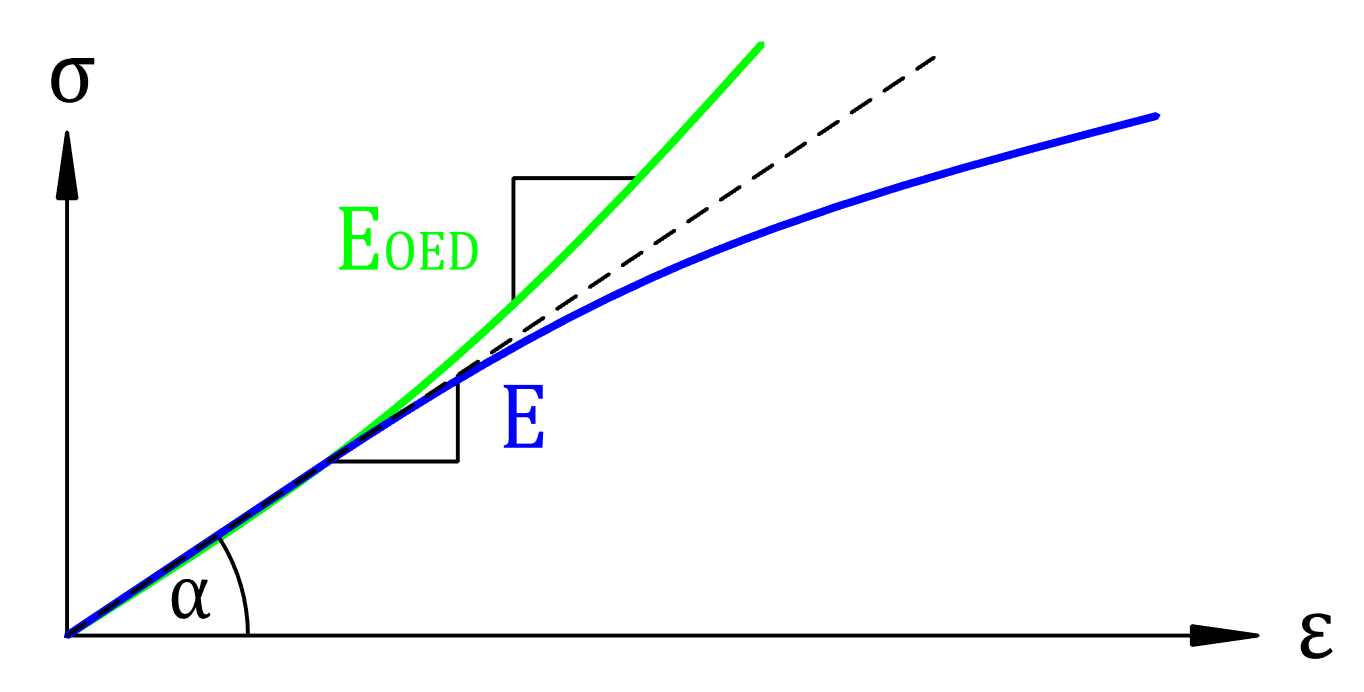
\includegraphics[width=0.5\linewidth,keepaspectratio]{papers/spannung/Grafiken/DiagrammOedometer-Versuch.png}
	\caption{Diagramm Charakteristik verschiedener Elastizitätsmodule bei gleichem Material}
	\label{fig:DiagrammOedometer-Versuch}
\end{figure}